\documentclass{beamer}
\usetheme{CambridgeUS}
%Information to be included in the title page:
\institute{UNIVERSITATEA ”ALEXANDRU-IOAN CUZA” DIN IAȘI}
\title{Music Recognition Using Convolutional Neural Networks}
\\
\\
\author{{Absolvent: Vavilov Andrei} \\
{\and} \\
{Coordonator științific: Conf. Dr. Vitcu Anca} }
\date{Sesiunea: Iulie 2021}

\begin{document}

\frame{\titlepage}

\begin{frame}
\frametitle{Table of Contents}

\begin{itemize}
	\item Motivation
	\item Personal contributions
	\item Application architecture
	\item Demo
	\item Possible improvements
	\item Conclusion
	\item Bibliography
\end{itemize}
\end{frame}

\begin{frame}
\frametitle{Motivation}
In the age of big data and immense computational power, artificial intelligence
has come to be the new standard in the computer science field. Various types of data
can be understood, learnt, predicted and even produced by a well-tuned neuronal network,
making the principles of machine learning a must for a scientist nowadays.


Applications of neuronal networks can be found in any discipline: from medicine
to physics, social sciences and languages. The purpose of this thesis is to depict how
artificial intelligence can find its place and purpose in a previously profoundly human
field: art.
\end{frame}

\begin{frame}
\frametitle{Personal contributions}
Numerous attempts of creating a medium between artificial intelligence and other
disciplines have been made since the rise of this field. Arts, especially music, is no exception.
The particularity of the current thesis is the approach we had in completing the
task: implementing from scratch the neural network framework, and, implicitly, understanding
the mathematical and theoretical subtleties of it, as well as creating the
visual aid which aims to touch on (although briefly) 3D animations.
\end{frame}

\begin{frame}
\frametitle{Application architecture}
The application is divided into three parts:
\begin{itemize}
	\item The Neuronal Network Engine
	\item The User Input Handling and Processing
	\item The Application-User interaction via the GUI
\end{itemize}
The application architecture is illustrated in the below figure:
\begin{center}
	\centering
	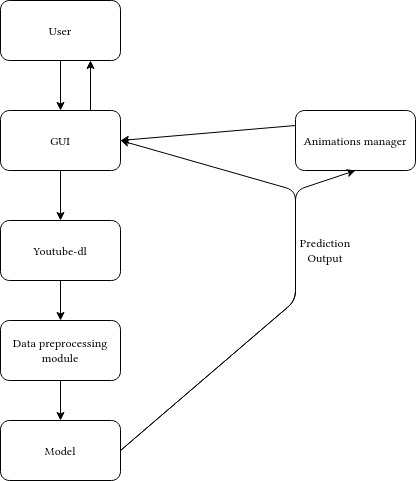
\includegraphics[width = 1.5in]{images/fac.png}
	\centerline{\captionof{Figure: Application architecture}}
	\label{uc1}
	\end{center}
\end{frame}
\begin{frame}
\frametitle{Demo}
\end{frame}

\begin{frame}
\frametitle{Possible improvements}
Given that the problem the application solves is a binary one, a possible improvement is
to increase the number of classes in order to represent multiple instruments.
One possible scenario would be distinguishing between the instruments of an orchestra.
Obviously that implies creating the corresponding 3D animations.
On the same note another improvement would refer to implementing GPU numeric
operations support in order to improve the speed of the training process which is
\end{frame}

\begin{frame}
\frametitle{Conclusion}
The three constituent parts of the application  form a project that serves its purpose:
to both create a middle way between arts and computer science, making the applications
of machine learning interesting, yet engaging and to get a deeper understanding, by
implementing the neuronal network framework from scratch, of the mathematical and theoretical
subtleties of artificial intelligence.
The application succeeds in creating the liaison between an intuitive and friendly
user experience and the complex background of the custom machine learning framework.
Therefore, we believe that the current thesis corresponds with the initial ambition of the project.
\end{frame}

\begin{frame}
\frametitle{Bibliography}
\begin{itemize}
	\item Harrison Kinsley and Daniel Kukieła. Neural Networks from Scratch in Python.
2020.
	\item Seth Adams. “Audio Classification”. In: (2020).

	\item Erik Lindernoren. “Machine Learning From Scratch”. In: (2019).

\end{itemize}
\end{frame}
\end{document}
